\documentclass{article}

\usepackage{times}
\usepackage{geometry}
\geometry{a4paper,left=0.6cm,right=0.7cm,top=1.5cm,bottom=1cm,columnsep=0.8cm}

\usepackage{fontawesome}          % icônes de base seulement
\usepackage[hidelinks]{hyperref}
\usepackage{multicol}
\usepackage{tikz}
\usepackage{hyphsubst}
\usepackage{moresize}
\usepackage{hyphenat}
\usepackage{tabularx}
\usepackage{ragged2e}
\usepackage{xcolor}
\usepackage{enumitem}
\usetikzlibrary{calc, positioning}
\newcolumntype{Y}{>{\RaggedRight\arraybackslash}X}

% icônes manquantes -> puce
\makeatletter
\@for\sym:=faBrain,faMicrochip,faHandshakeO,faTools,faNetworkWired,%
             faDatabase,faServer,faGit,faUsers,faComments,faCalendar,faGroup\do{%
  \@ifundefined{\sym}{\expandafter\newcommand\csname\sym\endcsname{\textbullet}}{}}
\makeatother

% couleurs
\definecolor{maincolor}{HTML}{f0fafc}
\definecolor{seccolor}{HTML}{ffffff}
\definecolor{gray}{HTML}{8c94a9}
\definecolor{sidetext}{HTML}{59cee5}

% bande latérale bleue
\usepackage{eso-pic}
\AddToShipoutPictureBG{%
  \begin{tikzpicture}[remember picture,overlay]
    \fill[maincolor] (current page.north west) rectangle
                     ([xshift=0.3\paperwidth] current page.south west);
  \end{tikzpicture}%
}

% listes
\setlist[itemize]{itemsep=-2pt,topsep=0pt,leftmargin=1.08cm}
\renewcommand{\labelitemi}{\textcolor{sidetext}{\footnotesize$\bullet$}}

\setlength{\parindent}{0pt}
\usepackage{paracol}
\columnratio{0.3}

\begin{document}
\pagestyle{empty}

\begin{paracol}{2}
% ────────────────────────────────────────
% Colonne gauche
% ────────────────────────────────────────
\color{sidetext}
\vspace*{-0.5cm}

\noindent
\begin{minipage}{\linewidth}
  \centering
  \begin{tikzpicture}
    \clip (0,0) circle (1.5cm) node[anchor=center]
      {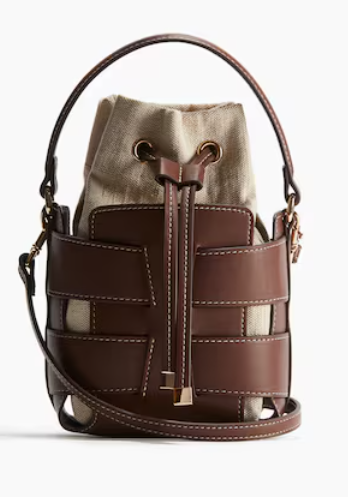
\includegraphics[width=3cm]{57916fcb492c4adfbca9309d34819490.png}};
  \end{tikzpicture}

  \vspace{3mm}
  {\color{black}\LARGE \textbf{Judikael Mourouvin}}

  \vspace{1mm}
  {\large Technicien informatique \& marketing digital}

  \vspace{3mm}
  {\color{gray}\rule{\linewidth}{0.4pt}} \\
\end{minipage}

% ── Coordonnées
\begin{tabular}{@{}c l}
  \faPhone &
  \begin{tabular}[t]{@{}l@{}}
    {\color{gray}Téléphone} \\ +590 0690 91 14 48
  \end{tabular} \\
  \\
  \faLinkedin &
  \begin{tabular}[t]{@{}l@{}}
    {\color{gray}LinkedIn} \\
    \href{}{Mon LinkedIn}
  \end{tabular} \\
  \\
  \faMapMarker &
  \begin{tabular}[t]{@{}l@{}}
    {\color{gray}Adresse} \\ Route de Cocoyer \\ 97190 Gosier
  \end{tabular} \\
  \\
  \faEnvelope &
  \begin{tabular}[t]{@{}l@{}}
    {\color{gray}Email} \\
    \href{mailto:jkmou971@gmail.com}{jkmou971@gmail.com}
  \end{tabular} \\
\end{tabular}

\vspace{2mm}
{\color{gray}\rule{\linewidth}{0.4pt}} \\

% ── Langues --------------------------------------------------------
{\color{black}{Langues}}

\vspace{2mm}
\begin{itemize}[leftmargin=*]
\item English - \textcolor{gray}{}
\item Espagnol - \textcolor{gray}{}\end{itemize}          % ← le placeholder va contenir \begin{itemize}…\end{itemize}

{\color{gray}\rule{\linewidth}{0.4pt}} \\

% ── Compétences ----------------------------------------------------
\vspace{2mm}
{\color{black}{Compétences Clés}}

\vspace{2mm}
\begin{itemize}[leftmargin=*]
\item Administration
\item Réseaux
\item Maintenance
\item Support
\item Configuration
\item Marketing
\item Diagnostic\end{itemize}              % ← idem, une vraie liste
\vspace{2mm}
{\color{gray}\rule{\linewidth}{0.4pt}} \\

% ── Centres d'intérêt
\vspace{2mm}
{\color{black}{Centres d’intérêt}}

\vspace{2mm}
\begin{itemize}[leftmargin=*]
\item Lectur
\item Sports
\item Musique
\item Voyage
\end{itemize}     % ← simple itemize ou tabular

\vfill
~

% ────────────────────────────────────────
\switchcolumn
% Colonne droite
% ────────────────────────────────────────
\color{black}

% ── Profil
\textcolor{black}{\Large \textbf{Profil Professionnel}} \\[2pt]
Professionnel passionné par l’informatique et le marketing digital, je maîtrise la configuration de postes, la maintenance et le diagnostic d’incidents. Mon année d’alternance à la DSI de la Mairie du Gosier m’a permis de piloter des projets numériques et d’accompagner les utilisateurs. Rigoureux et orienté résultats, je souhaite désormais mettre mes compétences au service de nouveaux défis à temps plein. Mon objectif : optimiser vos systèmes et soutenir votre stratégie digitale. \\[8pt]

% ── Expérience
\textcolor{black}{\Large \textbf{Expérience Professionnelle}} \\[2pt]
\colorbox{maincolor}{%
  \begin{minipage}{\linewidth}
    \noindent
    \textbf{Alternant en Marketing Digital}\hfill 2023-2024\\
    Mairie du Gosier – DSI\\[-0.3em]
    \begin{itemize}[leftmargin=*]
      \item Coordonné des projets numériques municipaux, garantissant leur déploiement conforme aux objectifs stratégiques. \item Analysé les besoins des usagers et déployé des solutions adaptées, améliorant l’efficacité du service. \item Assuré support et formation, favorisant l’adoption des outils digitaux par les utilisateurs.
    \end{itemize}
  \end{minipage}}

\vspace{3mm}

\colorbox{maincolor}{%
  \begin{minipage}{\linewidth}
    \noindent
    \textbf{Animateur de la zone informatique}\hfill 2022-2023\\
    Pôle Emploi, Gosier\\[-0.3em]
    \begin{itemize}[leftmargin=*]
      \item Fournit assistance et support aux demandeurs d’emploi, réduisant les temps de résolution d’incidents. \item Configuré et maintenu les postes de travail, assurant leur disponibilité continue. \item Diagnostiqué et résolu les pannes matérielles et logicielles, sécurisant le parc informatique.
    \end{itemize}
  \end{minipage}}

\vspace{3mm}

\colorbox{maincolor}{%
  \begin{minipage}{\linewidth}
    \noindent
    \textbf{Stagiaire Informaticien}\hfill 2020-2021\\
    Numerika, Baie-Mahault\\[-0.3em]
    \begin{itemize}[leftmargin=*]
      \item Installé et entretenu les équipements informatiques, garantissant leur performance. \item Assuré le support technique de premier niveau, améliorant la satisfaction des utilisateurs.
    \end{itemize}
  \end{minipage}}   % ← blocs \colorbox{maincolor}{\begin{minipage}…}

\vspace{8mm}

% ── Formation
\textcolor{black}{\Large \textbf{Formation}} \\[2pt]

\begin{tabularx}{\linewidth}{@{}c  >{\RaggedRight\arraybackslash}X
                             >{\raggedleft\arraybackslash}p{0.25\linewidth}@{}}
\textcolor{sidetext}{\faGraduationCap} &
Bachelor Marketing Digital &
2023-2024 \\
& CFA IUTS & \\   % ligne de l’établissement
\end{tabularx}
\begin{itemize}[leftmargin=*]
  \item Méthodes de conception et déploiement de stratégies digitales multicanales.
  \item Analyse de données, référencement et gestion de contenu web.
\end{itemize}
\vspace{3mm}

\begin{tabularx}{\linewidth}{@{}c  >{\RaggedRight\arraybackslash}X
                             >{\raggedleft\arraybackslash}p{0.25\linewidth}@{}}
\textcolor{sidetext}{\faGraduationCap} &
BTS Système Numérique – option Informatique et Réseaux &
2019-2021 \\
& Lycée de Chevalier Saint Georges, Abymes & \\   % ligne de l’établissement
\end{tabularx}
\begin{itemize}[leftmargin=*]
  \item Architecture des réseaux et administration de systèmes.
  \item Maintenance matérielle et logicielle, support aux utilisateurs.
\end{itemize}       % ← lignes tabular par diplôme

\end{paracol}
\end{document}

